\section{Introduction}

Multi-objective Optimization Problems (MOPs)~\cite{miettinen1999nonlinear} are problems composed of two or more functions which must be simultaneously optimized by the same set of parameters. This composition is characterized by a set of conflicting objective functions resulting in a set of optimal compromise solutions. 

These $m$ multiple objective functions must be optimized simultaneously:

\begin{align}\label{min_problem}
\text{minimize} f(x) = (f_1(x), ..., f_{m}(x)), \text{ with $x \in \mathbb{R}^{D}$},
\end{align}

where $m$ is the number of objective functions and $\mathbb{R}^m$ is the objective function space. $x \in \mathbb{R}^{D} = \{x_1, x_2, ..., x_D\}$ is a D-dimensional vector and it represents a candidate solution with ${D}$ variables, $f: \mathbb{R}^{D} \rightarrow \mathbb{R}^{m}$ is a vector of objective functions.% and $\Omega$ is the feasible decision space. $\Omega$ is defined as:

%\begin{align}
%\Omega =\{x \text{ in } \mathbb{R}^{n_v} | g_i(x) \leq 0 \text{ } \forall_i \text{ and } h_i(x) = 0 \text{ } \forall_j \},
%\end{align}
These objectives often conflict with each other, as there is no point in $\mathbb{R}^{D}$ that minimizes all the objectives at the same time. Consequently, the goal of the MOP optimization algorithm is to find the approximate sets of solutions that balance the different objectives in an optimal way.

Given two solutions vectors $u, v$ in $\mathbb{R}^{D}$, $u$  Pareto-dominates $v$, denoted by $f(u) \prec f(v)$, if and only if $f_k(u) \leq f_k(v), \forall_k \in \{1,..., m\}$ and $ f(u) \neq f(v)$. Likewise, a solution $x \in \mathbb{R}^{D}$ is considered Pareto-Optimal if there exists no other solution $y \in \mathbb{R}^{D}$ such that $f(y) \succ f(x)$, i.e., if $x$ is non-dominated in the feasible decision space. A non-dominated solution exists if no other solution provides a better balance in all objectives.

Consequently, the set of all Pareto-Optimal solutions is known as the Pareto-Optimal Set (PS), while the image of this set is referred to as the Pareto-optimal Front (PF).\\

\begin{equation}
PS = \{x \in \mathbb{R}^{D} | \nexists y \in \mathbb{R}^{D} : f(y) \succ f(x)  \},
\end{equation}

\begin{equation}
PF = \{f(x) | x \in PS \}.
\end{equation}

Multi-objective evolutionary algorithms (MOEAs) are one of the most widely used groups of algorithms for finding approximations to the PF of a MOP. They are characterized by their ability to find good approximations to PF in a single run~\cite{zhou2011multiobjective}. In recent years, there has been an increasing interest in studying MOEAs and with a primary concern of improving their general performance. Among MOEAs, there are three major paradigms: Pareto domination-based approaches~\cite{deb2002fast},~\cite{zitzler2001spea2}; the indicator-based approaches~\cite{beume2007sms},~\cite{zitzler2004indicator} and the decomposition-based approaches~\cite{li2009multiobjective},~\cite{zhang2007moea}. 

In this study, we are interested in analyzing the Multi-objective Evolutionary Algorithm based on Decomposition framework, MOEA/D~\cite{zhang2007moea}. It represents a class of population-based meta-heuristics for solving Multi Objective Problems~\cite{trivedi2017survey}. In this framework, the original multi-objective problem is decomposed into simpler, single-objective subproblems by means of scalarizations which defines the weights vectors. Each subproblem is then evaluated and its utility value is calculated by an aggregation function given the related weight vector. In the original MOEA/D, all the subproblems have the same amount of computational resource (number of iteractions). 
%\begin{figure}[h]
%	\centering
%	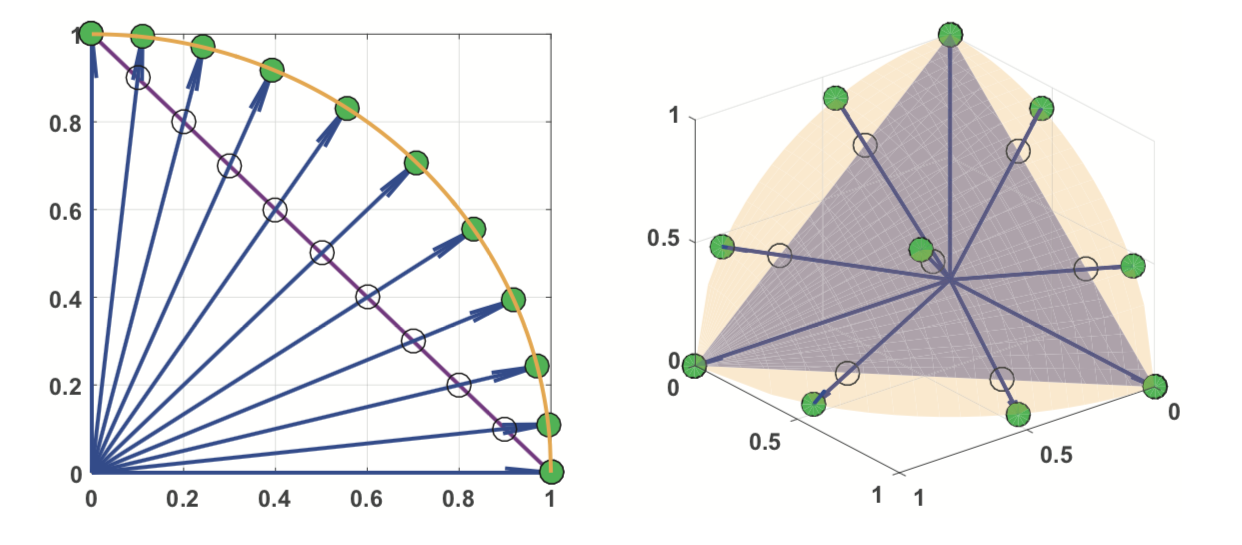
\includegraphics[width=0.55\textwidth]{img/decomp2.png}
%	\caption{A decomposition strategy generates weight vectors that defines the subproblems. Figure from~\cite{chugh2017handling}.}
%	\label{fig1}
%\end{figure}
%
%\begin{figure}[h]
%	\centering
%	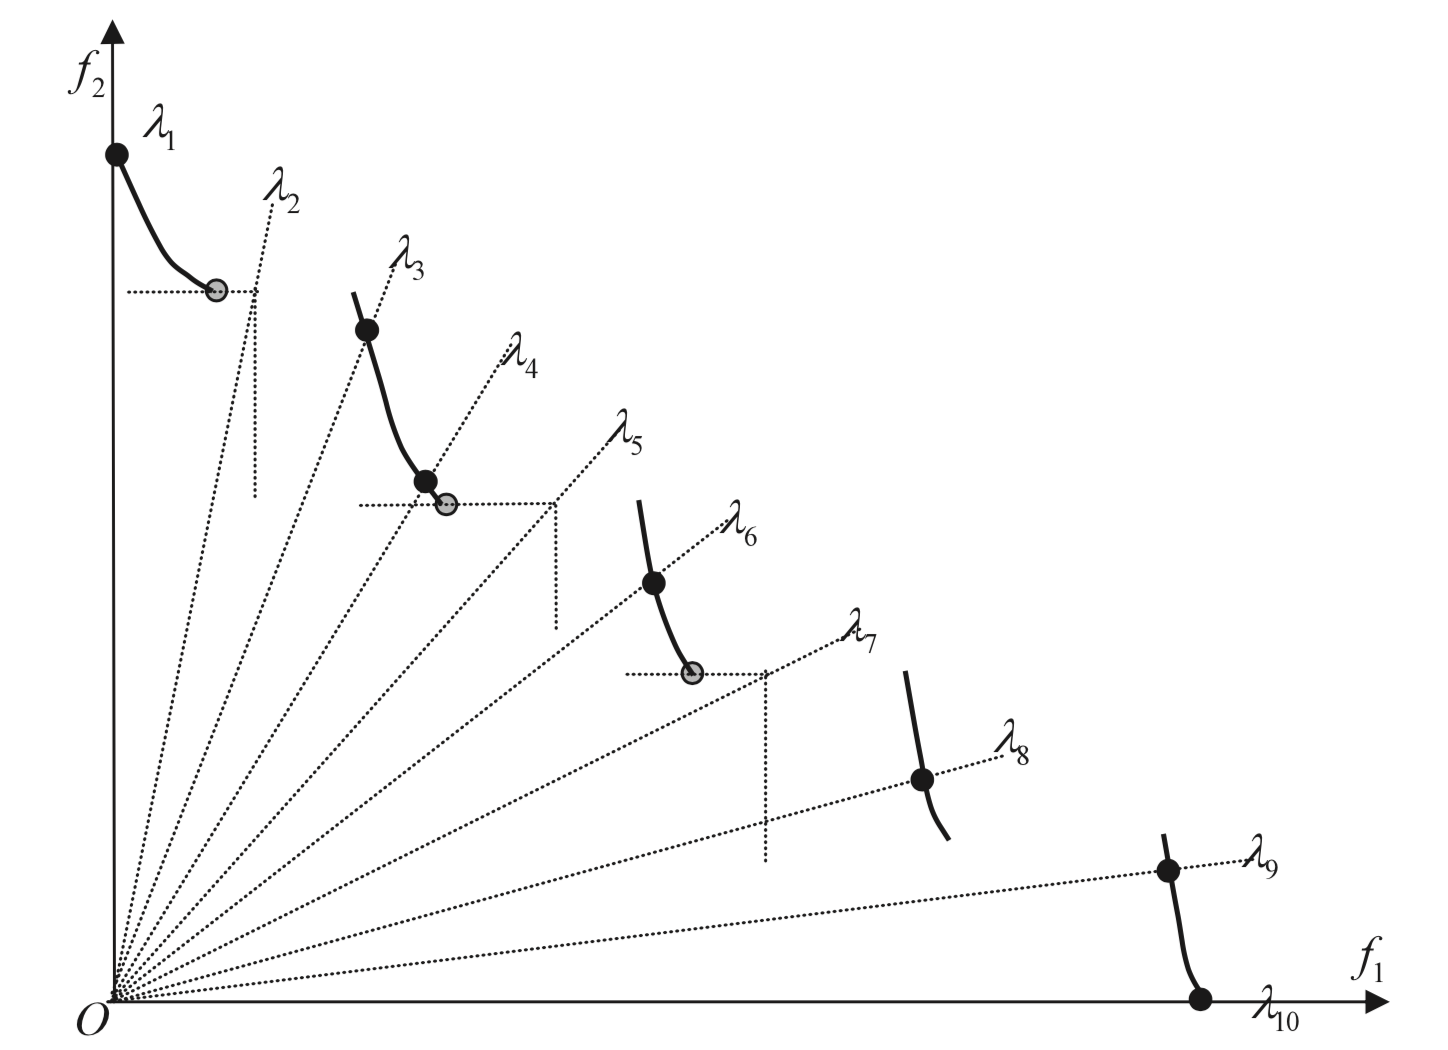
\includegraphics[width=0.43\textwidth]{img/harder_problems}
%	\caption{Distribution of optimal solutions of subproblems with uniform weight vectors on ZDT3. Figure from~\cite{li2015use}.}
%	\label{fig2}
%\end{figure}
%
%
%\begin{figure}[h]
%	\centering
%	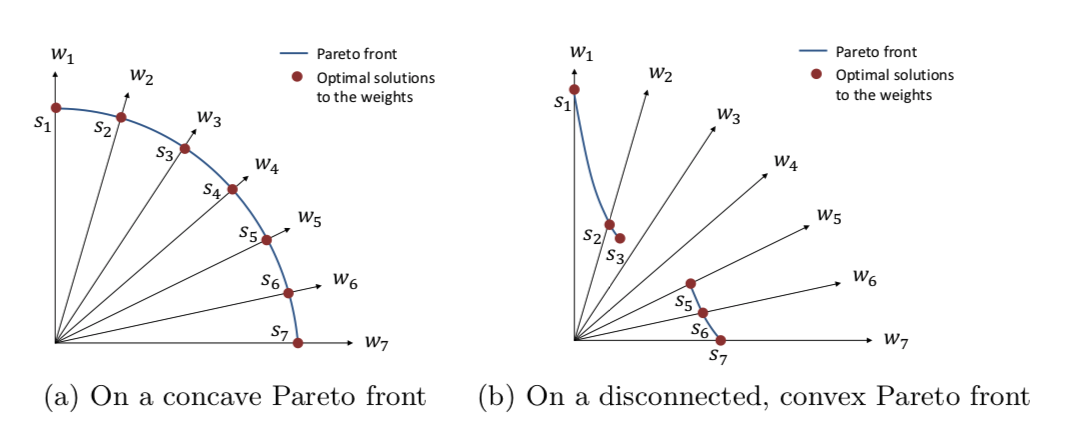
\includegraphics[width=0.53\textwidth]{img/harder_problems2}
%	\caption{An example that uniformly distributed weights may lead to different distributions of optimal solutions. (a) Solutions $s_1$ to $s_7$ are the optimal solutions of weights $w_1$ to $w_7$, respectively. (b) Solutions $s_1$,$s_2$,$s_3$,$s_6$ and $s_7$ are the optimal solutions of $w_1$,$w_2$,$w_3$,$w_6$ and $w_7$, respectively, while solution $s_5$ is the optimal solution of $w_4$ and $w_5$.Figure from~\cite{li2017weights}}
%	\label{fig3}
%\end{figure}



%It represents a class of population-based meta-heuristics for solving MOPs. Many other algorithms exists as NSGA-2(3), MOEA/Ds, IBEA, SPEA2, DEMO.
%interest of the PF. This duality between regions may lead to an unbalanced exploration of the search space, since it would be preferable to focus only on subproblems related to regions of interest.

Although researchers have not studied this problem in much detail, there have been some works that have discussed this matter. One way to address this problem is to adjust the behavior of the algorithm in an online manner to suit the problem in question~\cite{hinterding1997adaptation},~\cite{de2007parameter},~\cite{meyer2007self},~\cite{zhang2009performance},~\cite{kramer2010evolutionary},~\cite{zhang2012survey}~\cite{cai2015external}. All algorithmic components can be tunned adaptively and often feedback information is needed for these adaptation strategies. 

Another way, is  allocating different number of evaluations to the subproblems based on some priority function. In a few recent works, a utility function is used to prioritize resources given to subproblems that contribute more to the algorithm's search.  In the works of Zhang et al.~\cite{zhang2009performance} and Zhou et al.~\cite{zhou2016all} a utility function was proposed aiming to prioritize solutions based on a historical convergence information during different generations. Another approach was implemented in~\cite{kang2018collaborative}, where the utility function was based on the presence of a solution from the main population on a secondary population.

The aim of this study is to explore the relationship between subproblems and utility functions. Here, we propose a new methodology for defining these priority functions given a diversity metric. This studies examines the integration of an online diversity metric based on a geometrical perspective~\cite{gee2015online} as direct way to define the utility function. Unfortunately, a full discussion of diversity metrics as utility function lies beyond the scope of this study.
%The main contributions of this paper can be summarized as follows:

%\begin{itemize}
%	\item blablabla
%	\item blebleble
%	\item bliblibli
%\end{itemize}

%This work is divided in sections and subsections according to this and that.

